\documentclass[12pt,a4paper]{article}
\usepackage{amsmath,amscd,amsbsy,amssymb,latexsym,url,bm,amsthm}
\usepackage{epsfig,graphicx,subfigure}
\usepackage{enumitem,balance}
\usepackage{wrapfig}
\usepackage{mathrsfs,euscript}
\usepackage[usenames]{xcolor}
\usepackage{hyperref}
\usepackage[vlined,ruled,linesnumbered]{algorithm2e}
\usepackage{float}
\hypersetup{colorlinks=true,linkcolor=black}

\newtheorem{theorem}{Theorem}
\newtheorem{lemma}[theorem]{Lemma}
\newtheorem{proposition}[theorem]{Proposition}
\newtheorem{corollary}[theorem]{Corollary}
\newtheorem{exercise}{Exercise}
\newtheorem*{solution}{Solution}
\newtheorem{definition}{Definition}
\theoremstyle{definition}

\renewcommand{\thefootnote}{\fnsymbol{footnote}}

\newcommand{\postscript}[2]
 {\setlength{\epsfxsize}{#2\hsize}
  \centerline{\epsfbox{#1}}}

\renewcommand{\baselinestretch}{1.0}

\setlength{\oddsidemargin}{-0.365in}
\setlength{\evensidemargin}{-0.365in}
\setlength{\topmargin}{-0.3in}
\setlength{\headheight}{0in}
\setlength{\headsep}{0in}
\setlength{\textheight}{10.1in}
\setlength{\textwidth}{7in}
\makeatletter \renewenvironment{proof}[1][Proof] {\par\pushQED{\qed}\normalfont\topsep6\p@\@plus6\p@\relax\trivlist\item[\hskip\labelsep\bfseries#1\@addpunct{.}]\ignorespaces}{\popQED\endtrivlist\@endpefalse} \makeatother
\makeatletter
\renewenvironment{solution}[1][Solution] {\par\pushQED{\qed}\normalfont\topsep6\p@\@plus6\p@\relax\trivlist\item[\hskip\labelsep\bfseries#1\@addpunct{.}]\ignorespaces}{\popQED\endtrivlist\@endpefalse} \makeatother

\begin{document}

\noindent

%========================================================================
\noindent\framebox[\linewidth]{\shortstack[c]{
\Large{\textbf{Lab04-Matroid}}\vspace{1mm}\\
CS214-Algorithm and Complexity, Xiaofeng Gao, Spring 2021.}}
\begin{center}
\footnotesize{\color{red}$*$ If there is any problem, please contact TA Haolin Zhou.}

% Please write down your name, student id and email.
\footnotesize{\color{blue}$*$ Name:\underline{Xin Xu}  \quad Student ID:\underline{519021910726} \quad Email: \underline{xuxin20010203@sjtu.edu.cn}}
\end{center}

\begin{enumerate}
\item \textit{Property of Matroid.} 
\begin{enumerate}
	\item
	Consider an arbitrary undirected graph $ G=(V,E) $. Let us define $ M_{G}=(S,C) $ where $ S=E $ and $ C=\left\{I \subseteq E \mid\left(V, E \backslash I\right) \text { is connected}\right\} $. Prove that $ M_{G} $ is a \textbf{matroid}.\par
	    \begin{proof}
	        \textbf{hereditary.} Let $B\in C$, and $A\subset B$. So, $(E \backslash B)\subset (E \backslash A)$. Since $(E \backslash B)$ is connected, $(E \backslash A)$ is connected.
			\\\textbf{exchange property.} Let $B,A\in C$ and $|A|<|B|$. We will prove exchange property by contradiction. The graph $(E\backslash A)$ must have more than one edges to connect the same two components of graph $G$. Otherwise, $(E\backslash A)$ only have $v-1$ edges, and $v=\text{the number of vertexes}$. In this case, $|A|$ is of the largest cardinality among all elements of $C$,
			                            which is contradictory to our hypothesis that $|A|<|B|$. Additionally, $B$ must contain at least one edge $e$ in $(E\backslash A)$ to connect the same two components. If not, $(E\backslash B)$ must hold the same edges of $(E\backslash A)$ except for the single edge connecting two components. But for the single edge, the total number is fixed, which means $|(E\backslash B)|\text{ is at least the same with} |(E\backslash A)|$ as a result,
										meaning $|B|\leqslant |A|$ too. So, we just pick this edge $e$ in $B$, and $A\cup \{e\}\in C$.
	    \end{proof}
	\item
	Given a set $A$ containing $n$ real numbers, and you are allowed to choose $k$ numbers from $A$. The bigger the sum of the chosen numbers is, the better. What is your algorithm to choose? Prove its correctness using \textbf{matroid}.\par
	\textbf{Remark:} Denote $\mathbf{C}$ be the collection of all subsets of $A$ that contains no more than $k$ elements. Try to prove $(A,\mathbf{C})$ is a matroid.\par
	    \begin{solution}
	        \textbf{algorithm.} Everytime choosing the largest number $x$ in $A$, and let $A=A\backslash x$. Repeat this process for $k$ times.
			\\\textbf{proof.} Denote $\mathbf{C}$ be the collection of all subsets of $A$ that contains no more than $k$ elements. And we will try to prove $(A,\mathbf{C})$ is a matroid. \textbf{hereditary:} Let $B\in \mathbf{C}$, and $D\subset B$. So $D$ is a set with elements less than $k$, which is clearly an element of $\mathbf{C}$.
			\textbf{exchange property.} Let $B,D\in \mathbf{C}$ and $|D|<|B|$. For every $x\in B\backslash D,D\cup \{x\}$ is a subset of $A$, whose cardinality is no more than $k$. So, $D\cup \{x\}\in \mathbf{C}$. Above all, $(A,\mathbf{C})$ is a matroid, and the greedy algorithm is the optimal method for maximization problem. 
	    \end{solution}

\end{enumerate}
\item \textit{Unit-time Task Scheduling Problem.} Consider the instance of the \textbf{Unit-time Task Scheduling Problem} given in class. 
    \begin{enumerate}
        \item Each penalty $\omega_{i}$ is replaced by $80-\omega_{i}$. The modified instance is given in Tab.~\ref{tab:1}. Give the final schedule and the optimal penalty of the new instance using Greedy-MAX.
		\begin{table}[H]
			\setlength{\abovecaptionskip}{0.cm}
			\setlength{\belowcaptionskip}{0.5cm}
			\centering
			\caption{Task}
			\label{tab:1}			
			\begin{tabular}{|c|ccccccc|}
				\hline
				$ a_{i} $&1&2&3&4&5&6&7\\
				\hline
				$ d_{i} $&4&2&4&3&1&4&6\\
                \hline
                $ \omega_{i} $&10&20&30&40&50&60&70\\
				\hline
			\end{tabular}
		\end{table}
	        \begin{solution}
	            \textbf{the final schedule.} The order is $a_5,a_4,a_6,a_3,a_7,a_1,a_2$. And the sequence of $a_6 \text{ and } a_3$ can be exchanged, which is the same of $a_1 \text{ and } a_2$.
				\\\textbf{the optimal penalty.} The penalty is the sum of $a_1$ and $a_2$, which is $w_1+w_2=30.$
	        \end{solution}
        \item Show how to determine in time $O(|A|)$ whether or not a given set $A$ of tasks is independent. (\textbf{Hint}: You can use the lemma of equivalence given in class)
 	        \begin{solution}
                \begin{algorithm}[H]
					\KwIn{a set $A$ of $n$ tasks.}
					\KwOut{Whether or not $A$ is an independent system.}
					
					\BlankLine
					\caption{IndependentSystem}\label{Alg-system}
		
					Sort $n$ elements by penalties so that $w_1\geqslant w_2\geqslant ...\geqslant w_{n-1}\geqslant w_n$\;
					An array $a[n+2]$;$sum\leftarrow 0$;$j\leftarrow 0$\;
					\For{$j \leftarrow 0$ \KwTo $n+1$}{
						$a[j]=0$\;
					}
					\For{$j \leftarrow 1$ \KwTo $n$}{
						$++a[d_j]$\;
					}
					$j\leftarrow 0$\;
					\While{$sum\leqslant j$}{
						$++j$\;
						$sum\leftarrow sum+a[j]$\;
						\If{$j==n+1$}{break\;}	
					}

					\If{$j<n+1$}{\Return false\;}
					
					\Return true\;
	
				\end{algorithm}
            \end{solution}
    \end{enumerate}

\item \textit{MAX-3DM.} Let $X$, $Y$, $Z$ be three sets. We say two triples $\left(x_{1}, y_{1}, z_{1}\right)$ and $\left(x_{2}, y_{2}, z_{2}\right)$ in $X \times Y \times Z$ are \textit{disjoint} if $x_{1} \neq x_{2}$, $y_{1} \neq y_{2},$ and $z_{1} \neq z_{2}$. Consider the following problem:
    
    \begin{definition}[MAX-3DM] 
        Given three disjoint sets $X$, $Y$, $Z$ and a non-negative weight function $c(\cdot)$ on all triples in $X \times Y \times Z$, \textbf{Maximum 3-Dimensional Matching} (MAX-3DM) is to find a collection $\mathcal{F}$ of disjoint triples with maximum total weight.
    \end{definition}

    \begin{enumerate}
    	\item Let $D = X \times Y \times Z$. Define independent sets for MAX-3DM.
    	\item Write a greedy algorithm based on Greedy-MAX in the form of \emph{pseudo code}. \label{Item-Greedy}
    	\item Give a counter-example to show that your Greedy-MAX algorithm in Q.~\ref{Item-Greedy} is not optimal.
    	\item Show that: $\max\limits_{F \subseteq D} \frac{v(F)}{u(F)} \leq 3$. {\color{blue}(Hint: you may need Theorem~\ref{Thm-Intersect} for this subquestion.)} 
    	    \begin{solution}
    	        \begin{enumerate}
					\item Define $\mathbf{C}$ as: $\mathbf{C}=\{F\subseteq D|F \text{ is a collection of disjoint triples}\}$. And prove it an independent system. Let $B\in \mathbf{C}$ and $A\subset B$, it's clear that $A$ is a collection of disjoint triples. So, $A\in \mathbf{C}$.
					\item \begin{algorithm}[H]
						\KwIn{a set $D$ of $n$ triples.}
						\KwOut{A subset of $D$ with maximum weight.}
						
						\BlankLine
						\caption{MAX-3DM}\label{Alg-greedy}
			
						Sort $n$ triples by weights decreasingly so that $w_{d_1}\geqslant w_{d_2}\geqslant ...\geqslant w_{d_{n-1}}\geqslant w_{d_n}$\;
						$A\leftarrow \emptyset$\;
						\For{$j \leftarrow 1$ \KwTo $n$}{
							\If{$A\cup \{d_i\} \in \mathbf{C}$}{
								$A\leftarrow A\cup \{d_i\}$\;
							}
						}
						
						Output $A$;
		
					\end{algorithm}
					\item The picture of counter example is below. In this case, the greedy algorithm contains a total weight of $11$, while the optimal algorithm contains a total weight of $12$.
					\begin{figure}[htbp]
						\centering
						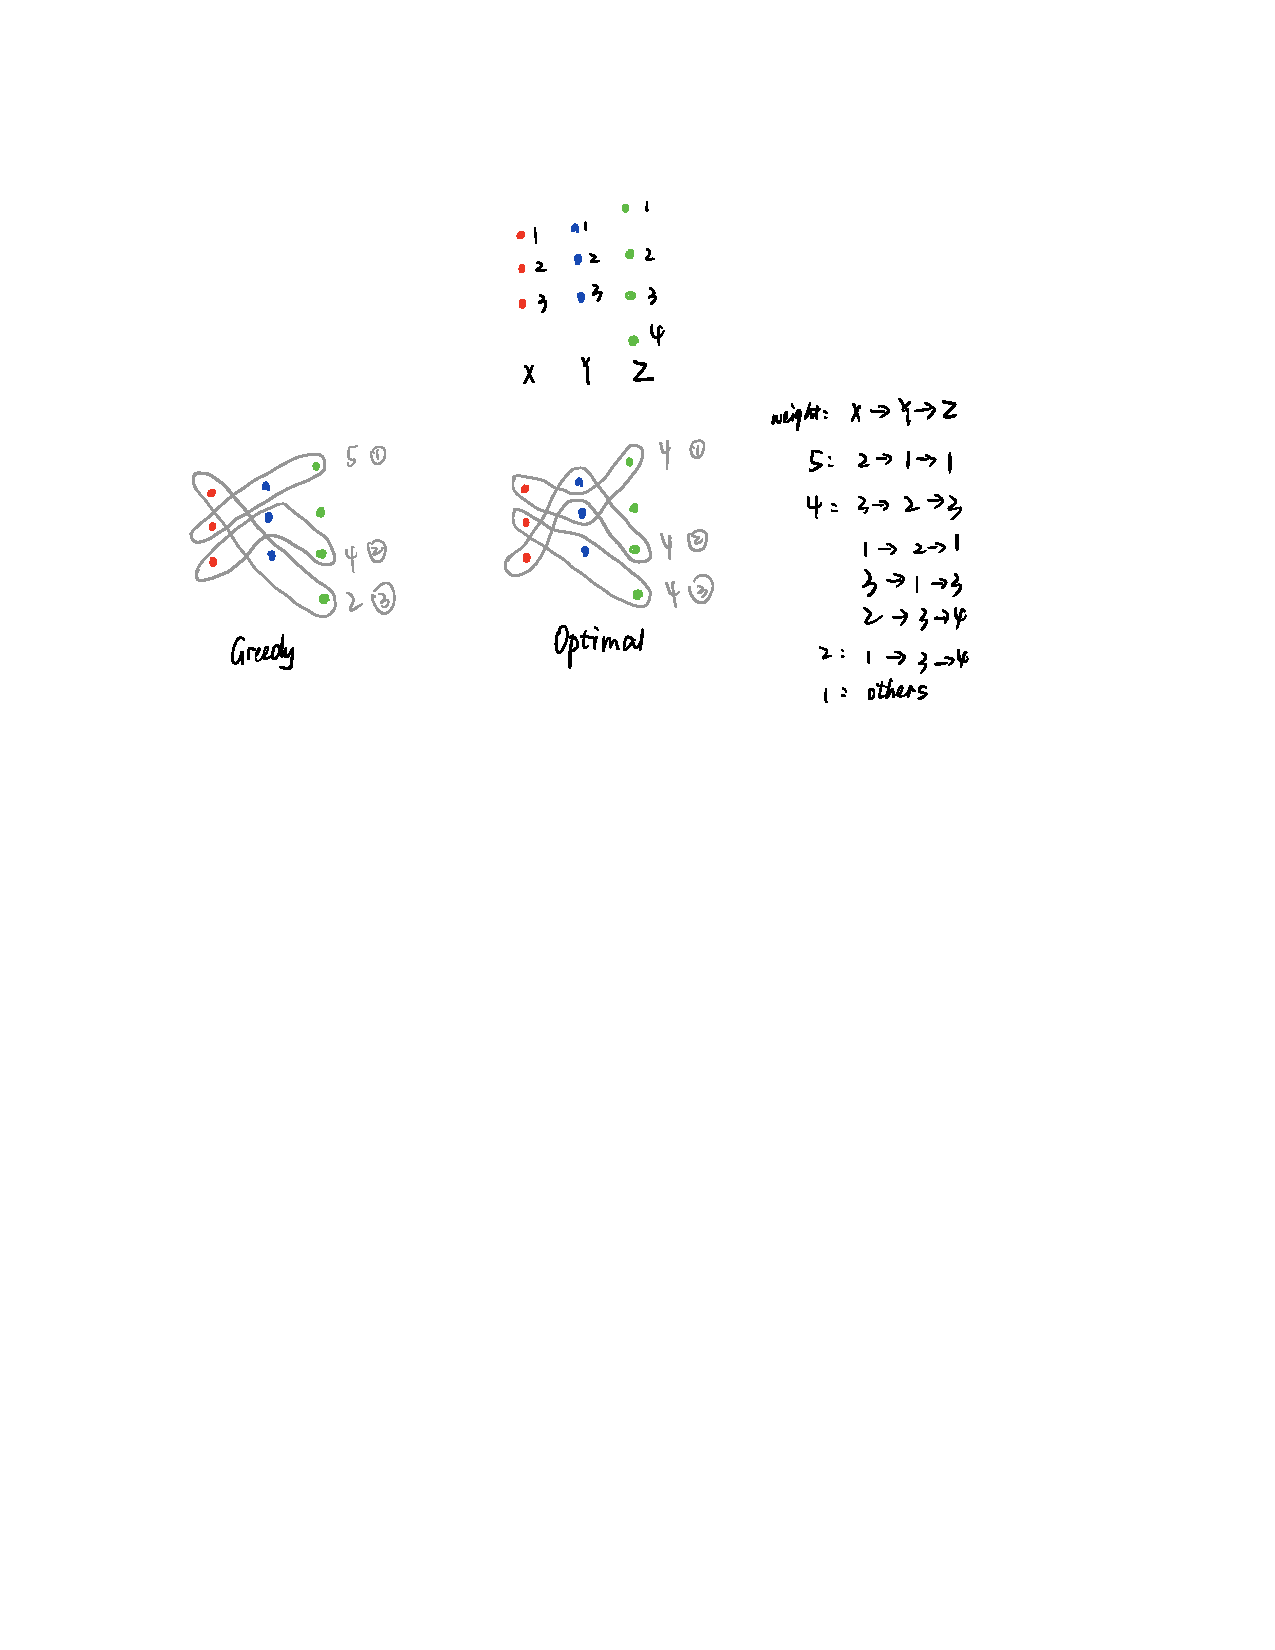
\includegraphics[width=0.4\textwidth]{Slide07-Matroid.pdf}
						\caption{The Counter Example}\label{counter-example}
					\end{figure}
					\item \begin{proof}The independent system $(D,\mathbf{C})$ is the intersection of $3$ matroids $(D,\mathcal{C}_{i}),1\leqslant i\leqslant 3$; that is, $\mathbf{C}=\bigcap_{i=1}^{3} \mathcal{C}_{i}$. 
					\\Define $\mathcal{C}_{1}$ as: $\mathcal{C}_{1}=\{F\subseteq D|F \text{ is a collection of triples that any } x_i\neq x_j \text{ if } i\neq j.\}$.
					\\Define $\mathcal{C}_{2}$ as: $\mathcal{C}_{2}=\{F\subseteq D|F \text{ is a collection of triples that any } y_i\neq y_j \text{ if } i\neq j.\}$.
					\\Define $\mathcal{C}_{3}$ as: $\mathcal{C}_{3}=\{F\subseteq D|F \text{ is a collection of triples that any } z_i\neq z_j \text{ if } i\neq j.\}$.
					\\And it's easy to prove that $\mathcal{C}_{1},\mathcal{C}_{2},\mathcal{C}_{3}$ are all matroids. According to \textbf{Theorem 1.}, $\max\limits_{F \subseteq D} \frac{v(F)}{u(F)} \leq 3$.
					\end{proof}
				\end{enumerate}
    	    \end{solution}
    \end{enumerate}
    \begin{theorem} \label{Thm-Intersect}
        Suppose an independent system $(E, \mathcal{I})$ is the intersection of $k$ matroids $\left(E, \mathcal{I}_{i}\right)$, $1 \leq i \leq k$; that is, $\mathcal{I}=\bigcap_{i=1}^{k} \mathcal{I}_{i}$. Then $\max\limits_{F \subseteq E} \frac{v(F)}{u(F)} \leq k$, where $v(F)$ is the maximum size of independent subset in $F$ and $u(F)$ is the minimum size of maximal independent subset in $F$.
    \end{theorem}    
\end{enumerate}

\vspace{20pt}

\textbf{Remark:} You need to include your .pdf and .tex files in your uploaded .rar or .zip file.

%========================================================================
\end{document}
